\section*{Chapter 7: Time Complexity}
\addcontentsline{toc}{section}{Chapter 7: Time Complexity}

\subsection*{7.1}

Answer each part TRUE or FALSE.

\begin{enumerate}[label=(\alph*), leftmargin=2.5em]

\item 2n = O(n). A

\item n log n = O(n2 ).

\item n2 = O(n). e. 3n = 2O(n) . n n

\item n2 = O(n log 2 n). f. 22 = O(22 ).

\end{enumerate}


\subsection*{7.2}

Answer each part TRUE or FALSE.

\begin{enumerate}[label=(\alph*), leftmargin=2.5em]

\item n = o(2n). d. 1 = o(n).

\item 2n = o(n2 ). e. n = o(log n).

\item 2n = o(3n ). f. 1 = o(1/n).

\end{enumerate}


\subsection*{7.5}

Is the following formula satisfiable?

(x $\lor$ y) $\land$ (x $\lor$ y) $\land$ (x $\lor$ y) $\land$ (x $\lor$ y)


\subsection*{7.7}

Show that NP is closed under union and concatenation.


\subsection*{7.9}

A triangle in an undirected graph is a 3-clique. Show that TRIANGLE $\in$ P, where TRIANGLE = \{hGi| G contains a triangle\}.


\subsection*{7.10}

Show that ALLDFA is in P.


\subsection*{7.14}

Show that P is closed under homomorphism iff P = NP.


\subsection*{7.17}

Call a regular expression star-free if it does not contain any star operations. Then, let EQSF-REX = \{hR, Si| R and S are equivalent star-free regular expressions\}. Show that EQSF-REX is in coNP. Why does your argument fail for general regular expressions?


\subsection*{7.23}

For a cnf-formula $\varphi$ with m variables and c clauses, show that you can construct in polynomial time an NFA with O(cm) states that accepts all nonsatisfying assignments, represented as Boolean strings of length m. Conclude that P $\neq$ NP implies that NFAs cannot be minimized in polynomial time.


\subsection*{7.27}

This problem is inspired by the single-player game Minesweeper, generalized to an arbitrary graph. Let G be an undirected graph, where each node either contains a single, hidden mine or is empty. The player chooses nodes, one by one. If the player chooses a node containing a mine, the player loses. If the player chooses an empty node, the player learns the number of neighboring nodes containing mines. (A neighboring node is one connected to the chosen node by an edge.) The player wins if and when all empty nodes have been so chosen. In the mine consistency problem, you are given a graph G along with numbers labeling some of G's nodes. You must determine whether a placement of mines on the remaining nodes is possible, so that any node v that is labeled m has exactly m neighboring nodes containing mines. Formulate this problem as a language and show that it is NP-complete.


\subsection*{7.28}

In the following solitaire game, you are given an m $\times$ m board. On each of its m2 positions lies either a blue stone, a red stone, or nothing at all. You play by removing stones from the board until each column contains only stones of a single color and each row contains at least one stone. You win if you achieve this objective. Winning may or may not be possible, depending upon the initial configuration. Let SOLITAIRE = \{hGi| G is a winnable game configuration\}. Prove that SOLITAIRE is NP-complete.


\subsection*{7.29}

Let SET-SPLITTING = \{hS, Ci| S is a finite set and C = \{C1 , . . . , Ck \} is a collection of subsets of S, for some k > 0, such that elements of S can be colored red or blue so that no Ci has all its elements colored with the same color\}. Show that SET-SPLITTING is NP-complete.


\subsection*{7.30}

Consider the following scheduling problem. You are given a list of final exams F1 , . . . , Fk to be scheduled, and a list of students S1 , . . . , Sl . Each student is taking some specified subset of these exams. You must schedule these exams into slots so that no student is required to take two exams in the same slot. The problem is to determine if such a schedule exists that uses only h slots. Formulate this problem as a language and show that this language is NP-complete.


\subsection*{7.32}

A subset of the nodes of a graph G is a dominating set if every other node of G is adjacent to some node in the subset. Let

DOMINATING-SET = \{hG, ki| G has a dominating set with k nodes\}.

Show that it is NP-complete by giving a reduction from VERTEX-COVER.


\subsection*{7.34}

Let U = \{hM, x, \#t i| NTM M accepts x within t steps on at least one branch\}. Note that M isn't required to halt on all branches. Show that U is NP-complete.


\subsection*{7.36}

Show that if P = NP, you can factor integers in polynomial time. (See the note in Problem 7.35.)


\subsection*{7.39}

You are given a box and a collection of cards as indicated in the following figure. Because of the pegs in the box and the notches in the cards, each card will fit in the

box in either of two ways. Each card contains two columns of holes, some of which may not be punched out. The puzzle is solved by placing all the cards in the box so as to completely cover the bottom of the box (i.e., every hole position is blocked by at least one card that has no hole there). Let PUZZLE = \{hc1 , . . . , ck i| each ci represents a card and this collection of cards has a solution\}. Show that PUZZLE is NP-complete.

\begin{figure}[h]

\centering

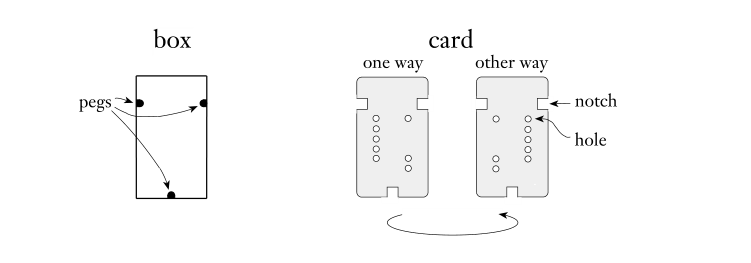
\includegraphics[width=0.72\textwidth]{chapters/assets/exercise_7_39_figure.png}

\caption*{Puzzle figure from Exercise 7.39}

\end{figure}


\subsection*{7.40}

Let

$MODEXP = \{\langle a, b, c, p\rangle \mid a, b, c,$ and $p$ are positive binary integers such that $a^b \equiv c \pmod p\}$.
Show that $MODEXP \in P$. (Note that the most obvious algorithm doesn't run in polynomial time. Hint: Try it first where $b$ is a power of 2.)


\subsection*{7.42}

Show that P is closed under the star operation. (Hint: Use dynamic programming. On input y = y1 · · · yn for yi $\in$ $\Sigma$, build a table indicating for each i $\le$ j whether the substring yi · · · yj $\in$ A$\ast$ for any A $\in$ P.)


\clearpage
